% !TEX root = ../main.tex

\chapter{基于势博弈的分布式任务分配方法}
\label{chap:pg}



\section{引言}
\label{pg:intro}

本章使用第\ref{chap:model}章中建立的空空导弹任务分配模型,设计了面向任务分配问题的势博弈模型(Potential Game, PG)框架。本章首先介绍了势博弈模型概念,并选择合适的函数作为智能体效用,初步建立了势博弈模型;接着针对任务分配中的约束问题,使用Lagrange乘子法对原始势博弈模型进行改进,并证明了模型的可行性与性能下界;然后,针对改进的势博弈模型,使用多种均衡求解算法进行模型求解;最后,通过仿真与对比实验验证了模型与算法的有效性。

%--------------------------------
%--------------------------------
\section{势博弈模型}
\label{pg:model}
在任务分配问题框架下,当所有导弹依据最大化自身效用的原则选择的目标不再发生变化时,则称所有导弹达到了均衡状态。博弈论中一个经典的均衡状态是纯纳什均衡,它表示一个任务分配解$a^*=(a_1^*,\dots,a_{n_m}^*)$,满足任意一个导弹不能通过独自改变任务提高自身效用。在具体阐述纳什均衡和势博弈概念前,除第\ref{chap:model}章使用的概念外,仍需要引入以下概念和符号。设$a_{-i}$表示除了导弹$\mathcal{M}_i$以外的其他导弹的分配集合,即
\[
a_{-i}=(a_1,\dots,a_{i-1},a_{i+1},\dots,a_{n_m}),
\]
利用该符号可将一组分配解表示为$(a_i,a_{-i})$。此外,可类似地定义$\mathcal{A}_{-i}$为
\[
\mathcal{A}_i:=\mathcal{A}_1 \times \dots \times \mathcal{A}_{i-1} \times \mathcal{A}_{i+1} \times \dots \times \mathcal{A}_{n_m} .
\]
设$U_{\mathcal{M}_i}(a)$或$U_{\mathcal{M}_i}(a_i,a_{-i})$表示导弹$\mathcal{M}_i$在分配$a$下的智能体效用,由此可得到纯纳什均衡的定义:
\begin{definition}[纯纳什均衡]
\label{pg:def:pureNash}
	若一个分配解$a^*$满足
	\begin{equation}
\label{pg:eq:pure_Nash}
	U_{\mathcal{M}_i}(a_i^*,a_{-i}^*)=\max_{a_i\in \mathcal{A}_i}U_{\mathcal{M}_i}(a_i,a_{-i}^*),\quad \forall \mathcal{M}_i \in \mathcal{M}.
\end{equation}
则称$a^*$是一个纯纳什均衡解。
\end{definition}

当所有导弹达到纯纳什均衡时,全局效用未必实现最大化;另一方面,在一些博弈场景下纯纳什均衡未必存在。因此,引入势博弈概念

\begin{definition}[有序势博弈与势博弈]
\label{pg:def:potentialGame}
	设一个博弈模型中的智能体效用函数为$U_{\mathcal{M}_i}(a),\mathcal{M}_i\in \mathcal{M}$,如果存在一个全局势函数$\phi(a):\mathcal{A} \mapsto \mathbb{R}$,满足对任意智能体$\mathcal{M}_i \in \mathcal{M}$,任意$a_{-i}\in \mathcal{A}_{-i}$,智能体$\mathcal{M}_i$的任意两个分配$a_i',a_i''\in \mathcal{A}_i$,有
	\begin{equation}
	\label{pg:eq:ordpg}
		U_{\mathcal{M}_i}(a_i',a_{-i})-U_{\mathcal{M}_i}(a_i'',a_{-i})>0 \Leftrightarrow \phi(a_i',a_{-i})-\phi(a_i'',a_{-i})>0,
	\end{equation}
	则该博弈模型是一个有序势博弈模型。在此基础上,若该全局势函数进一步满足:
	
	\begin{equation}
	\label{pg:eq:pgdef}
		U_{\mathcal{M}_i}(a_i',a_{-i})-U_{\mathcal{M}_i}(a_i'',a_{-i})=\phi(a_i',a_{-i})-\phi(a_i'',a_{-i}).
	\end{equation}
	则称该博弈模型为势博弈模型。若策略集$\mathcal{A}$是有限的,则称该势博弈为有限势博弈。
\end{definition}

由势博弈的定义可知,势博弈模型中的智能体效用变化会等同地反映在全局效用上,而在有序势博弈上,智能体效用与全局效用总是同向变化。易知势博弈是一种特殊的有序势博弈。有限势博弈模型有两点性质:

(1)有限势博弈至少存在一个纯纳什均衡;

(2)有限势博弈具有有限优化性质(finite improvement property, FIP)。

性质(1)保证了纯纳什均衡的存在性,因此对于任务分配问题,至少可以得到一个确定的解;性质(2)保证了任意智能体单方面提高自己效用的行为可以在有限时间内收敛到纯纳什均衡,从而保证了优化算法可在有限时间内收敛。




%--------------------------------
%--------------------------------
%-------------------------------------------------
%-----------------------------------------------

%--------------------------------
\section{面向任务分配问题的势博弈模型设计}
\label{pg:agent_utility}

\subsection{WLU效用函数}
\label{pg:wlu}
使用势博弈模型解决任务分配问题对导弹的智能体效用函数提出的要求是,满足

\begin{equation}
\label{pg:eq:pgU}
	U_{\mathcal{M}_i}(a_i',a_{-i})-U_{\mathcal{M}_i}(a_i'',a_{-i})=U_g(a_i',a_{-i})-U_g(a_i'',a_{-i}),
\end{equation}
使得所有导弹形成一个势博弈模型,其中$U_g(a)$即为式(\ref{model:eq:globalU})中定义的全局效用函数,因此在求解分配时所有导弹只需考虑最大化智能体效用便可实现全局效用最大化的目标。

一个显然而直接的思路是使用一致利益效用(Identical Interest Utility, IIU),其直接将全局效用作为智能体效用,但IIU的缺点在于需要计算所有任务效用后得到全局效用,因此本质上仍是集中式的方法。对IIU进行改进可以得到更分布化的有限区域效用(Range-Restricted Utility, RRU),RRU将智能体效用定义为所有该智能体参与的任务的效用之和,RRU可以使得智能体组成势博弈模型,但该模型的纳什均衡未必是最优的。此外,IIU和RRU有一个共同的问题在于如果存在大量的智能体同时参与大量的任务,由于IIU和RRU都是对一定数量的任务效用求和,此时一个智能体对任务的贡献微乎其微,即使它单方面改变决策,对该任务的效用改变可能很小,从而反映在智能体效用函数上的变化也很小。这对智能体的寻优和学习带来了很大难度。对此问题作出的改进是等份额效用(Equally Shared Utility, ESU),ESU用智能体参与的任务效用除以参与该任务的智能体总数,可以有效消除智能体数量带来的效用稀释作用,但ESU的局限在于只有当智能体之间不存在区别时才可以组成势博弈模型。

为了克服IIU和RRU的缺陷,且不局限于ESU的应用场景,本节采用的是WLU效用函数(Wonderful Life Utility),WLU将智能体效用函数定义为每个智能体对全局效用的边际贡献程度,其具体定义为:

\begin{equation}
\label{pg:eq:WLU1}
	U_{\mathcal{M}_i}(a_i,a_{-i}) = U_g(a_i,a_{-i}) - U_g(a_0,a_{-i}).
\end{equation}

由全局效用函数的定义式(\ref{model:eq:globalU})可将式(\ref{pg:eq:WLU1})改写为

\begin{equation}
\label{pg:eq:WLU2}
	U_{\mathcal{M}_i}(a_i,a_{-i}) = U_{\mathcal{T}_j}(a_i,a_{-i}) - U_{\mathcal{T}_j}(a_0,a_{-i}),\quad \text{if}\ a_i=\mathcal{T}_j.
\end{equation}

由式(\ref{pg:eq:WLU2})可知,WLU假设其他智能体不改变目标,智能体效用只与智能体自身的决策有关,因此WLU排除了冗余信息,比IIU和RRU优化能力更强。另外,下面的命题表明,使用WLU的博弈模型一定是势博弈模型。

\begin{proposition}[WLU可行性]
\label{pg:pro:mWLU}
	智能体效用函数为式(\ref{pg:eq:WLU2})的智能体集合组成的博弈模型是一个势博弈模型,且其势函数就是全局效用函数$U_g(a)$。
	
	\begin{proof}
	只需证明WLU满足式(\ref{pg:eq:pgU})即可。设$a_i,a_i' \in \mathcal{A}_i$,则有
	\begin{align}
		&\ U_{\mathcal{M}_i}(a_i,a_{-i}) - U_{\mathcal{M}_i}(a_i',a_{-i})\notag\\
		=&\ U_g(a_i,a_{-i}) - U_g(a_0,a_{-i}) - [U_g(a_i',a_{-i}) - U_g(a_0,a_{-i})]\notag\\
		=&\ U_g(a_i,a_{-i}) - U_g(a_i',a_{-i}) \notag
	\end{align}
	\end{proof}
\end{proposition}



\subsection{约束条件处理方法}
\label{pg:mWLU}

上述势博弈框架和智能体效用函数设计下,对于智能体选择任务并没有做出任何限制和约束,因此需要利用约束条件式(\ref{model:eq:simbmax})将势博弈的纳什均衡限制在可行解中。本节提出了基于Lagrange乘子法将有约束问题转化为无约束问题,并证明了在满足一定的条件下,新的无约束问题下获得的纳什均衡解均为原问题的可行解。

Lagrange乘子法是一种典型的处理含约束优化问题的方法,其将含约束问题转化为无约束问题,且可证明生成的新的无约束问题的最优解就是原问题的最优解。在势博弈模型下,结合全局效用函数的定义式(\ref{model:eq:simUg})以及约束条件式(\ref{model:eq:bmax}),将式(\ref{model:eq:taskU})任务效用函数$U_{\mathcal{T}_i}(a)$修正为:

\begin{equation}
\label{pg:eq:newTaskU}
	\widetilde U_{\mathcal{T}_j}(a) = U_{\mathcal{T}_j}(a) + \lambda [b_{\text{max}}^{(j)} - s_j]^-,
\end{equation}
其中$[x]^-=\min\{x,0\}$,$s_j$是第二章中定义的目标同为$\mathcal{T}_j$的导弹数量。由式(\ref{model:eq:globalU})得到修正后的全局效用函数为

\begin{equation}
\label{pg:eq:newglobalU}
		\widetilde U_g(a) = U_g(a) +  \lambda \sum_{j=1}^{n_t}[b_{\text{max}}^{(j)} - s_j]^-
	\end{equation}

再利用式(\ref{pg:eq:WLU2})提出的WLU效用函数计算修正后的智能体效用函数(modified WLU, mWLU)为

\begin{align}
\label{pg:eq:newAgentU}
	\widetilde U_{\mathcal{M}_i}(a_i,a_{-i}) &= \widetilde U_g(a_i,a_{-i}) - \widetilde U_g(a_0,a_{-i})\notag\\
	&= \widetilde U_{\mathcal{T}_j}(a_i,a_{-i}) - \widetilde U_{\mathcal{T}_j}(a_0,a_{-i}),\quad \text{if}\ a_i=\mathcal{T}_j.
\end{align}

下面需要验证mWLU的有效性,主要分为三部分:(1)满足mWLU效用的智能体能否组成势博弈模型;(2)该势博弈模型下得到的纳什均衡是否都满足原问题的约束;(3)该势博弈模型下得到的纳什均衡解的最优性。

%----------------------------
\subsubsection{势博弈成立条件}
\label{pg:mWLU:pgcondition}
为了验证mWLU函数的有效性,首先需要验证式(\ref{pg:eq:newAgentU})定义的智能体效用函数是否可以组成一个势博弈模型。设智能体效用函数为mWLU的智能体组成的组成的博弈模型为$\mathcal{G}=\{\mathcal{M},\mathcal{A},U_{\mathcal{M}}(a)\}$,实际上,可以得到以下结论:

\begin{proposition}[势博弈成立条件]
	$\mathcal{G}$是一个势博弈模型,其势函数为式(\ref{pg:eq:newglobalU})定义的全局效用函数。
	
	\begin{proof}
		只需证明全局效用函数$\widetilde U_g(a)$与式(\ref{pg:eq:newAgentU})定义的智能体效用函数$\widetilde U_{\mathcal{M}_i}(a_i,a_{-i})$满足式(\ref{pg:eq:pgU})即可。对任意$a_i',a_i'' \in \mathcal{A}_i$,$a'=(a_i',a_{-i}),a''=(a_i'',a_{-i})$,且$S',S''$分别为$a'$和$a''$对应的智能体分配集合,$s_j'$和$s_j''$分别为$S'$和$S''$中目标为$\mathcal{T}_j$的智能体数量。假设$a_i'=\mathcal{T}_j,\ a_i''=\mathcal{T}_k,\ j\neq k$,则有
		\begin{align}
			&\widetilde U_{\mathcal{M}_i}(a_i',a_{-i}) - \widetilde U_{\mathcal{M}_i}(a_i'',a_{-i})\notag\\
			= &\ [\widetilde U_g(a_i',a_{-i}) - \widetilde U_g(a_0,a_{-i})] - [\widetilde U_g(a_i'',a_{-i}) - \widetilde U_g(a_0,a_{-i})]\notag\\
			\label{pg:pf:eq:pg} = &\ \widetilde U_g(a_i',a_{-i}) - \widetilde U_g(a_i'',a_{-i})
		\end{align}
		所以满足mWLU效用的智能体可以组成一个势博弈模型,且势函数为全局效用函数$\widetilde U_g(a)$。
	\end{proof}
\end{proposition}

%--------------------------------
\subsubsection{纯纳什均衡可行性分析}
\label{pg:mWLU:pgexist}
在验证势博弈模型成立之后,下一步需要验证该势博弈模型所得到的纯纳什均衡是否是原问题的可行解,此处有以下结论:

\begin{proposition}[纳什均衡可行性]
\label{pg:pro:feasibility}
	当$\lambda$满足$\lambda > \lambda_0$时,若分配策略$a$是$\mathcal{G}$的一个纯纳什均衡,则$a$一定满足约束条件(\ref{model:eq:bmax})。其中
	\begin{equation}
		\lambda_0 = \max_{\substack{\mathcal{M}_i \in \mathcal{M}, \mathcal{T}_j \in \mathcal{T} \\ s_j > b_{\text{max}}^{(j)}}} \Bigg\{ \frac{U_{\mathcal{T}_j}(a_i,a_{-i}) - U_{\mathcal{T}_j}(a_i',a_{-i})}{s_j-b_{\text{max}}^{(j)}} \Bigg\}
	\end{equation}
	
	\begin{proof}
		设$a^*=(a_i^*,a_{-i}^*)$是势博弈模型$\mathcal{G}$的一个纯纳什均衡,但不满足约束条件(\ref{model:eq:bmax}),即存在$1\leq j \leq n_t, s_j^* > b_{\text{max}}^{(j)}$。对于参与任务$\mathcal{T}_j$的智能体之一$\mathcal{M}_k$,设$a_k^*=\mathcal{T}_j,a_k'=\mathcal{T}_l,\forall l \neq j$,则有
		\begin{align}
			&\widetilde U_{\mathcal{M}_k}(a_k^*,a_{-k}^*) - \widetilde U_{\mathcal{M}_k}(a_k',a_{-k}^*)\notag\\
		    =&\ \widetilde U_{\mathcal{T}_j}(a_k^*,a_{-k}^*) - \widetilde U_{\mathcal{T}_l}(a_k',a_{-k}^*)\notag\\
		    =&\ U_{\mathcal{T}_j}(a_k^*,a_{-k}^*) - \lambda(s_j^*-b_{\text{max}}^{(j)}) - [U_{\mathcal{T}_l}(a_k',a_{-k}^*) + \lambda[b_{\text{max}}^{(l)} - s_l']^-]\notag\\
		    \leq &\ U_{\mathcal{T}_j}(a_k^*,a_{-k}^*) - U_{\mathcal{T}_l}(a_k',a_{-k}^*) - \lambda(s_j^*-b_{\text{max}}^{(j)}) \notag \\
		    \leq &\ \max_{\mathcal{T}_j \in \mathcal{T}} \{U_{\mathcal{T}_j}(a_i^*,a_{-i}^*) - U_{\mathcal{T}_j}(a_i',a_{-i}^*)\} - \lambda_0(s_j^*-b_{\text{max}}^{(j)})
		\end{align}
		由$\lambda_0$的定义易知$\widetilde U_{\mathcal{M}_{k_0}}(a_{k_0}^*,a_{-{k_0}}^*) - \widetilde U_{\mathcal{M}_{k_0}}(a_{k_0}',a_{-{k_0}}^*) \leq 0$,这与$a^*$是纯纳什均衡的条件(\ref{pg:eq:pure_Nash})矛盾,因此$a^*$必然满足约束条件。
	\end{proof}
	
\end{proposition}

%---------------------
\subsubsection{纳什均衡最优性}
\label{pg:mWLU:pgoptimal}

在命题\ref{pg:pro:feasibility}下,势博弈模型$\mathcal{G}$的纳什均衡均为原问题的可行解,因此最后需要考察这些纳什均衡解的最优性。本节选择使用无秩序代价(Price of Anarchy, PoA)作为衡量纳什均衡性能的指标。设纯纳什均衡分配解为$a^*$,全局最优分配解为$a^{\text{opt}}$,则PoA的定义为全局最优效用和纳什均衡效用之比的上界:
\begin{equation}
\label{pg:eq:PoA}
	\mathrm{PoA}(\mathcal{G}) = \sup_{a^*} \Big\{ \frac{U_g(a^{\text{opt}})}{U_g(a^*)} \Big\}
\end{equation}

由PoA的定义可知,PoA越大,代表最差情况下纯纳什均衡效用越小,即意味着该势博弈模型的性能越差。关于本节建立的势博弈模型$\mathcal{G}$的PoA,我们可以用以下命题得到PoA的上界,从而保证了势博弈模型性能的下界。

\begin{proposition}
\label{pg:pro:PoA}
	势博弈模型$\mathcal{G}_{\text{PG}}$的PoA上界为
	\begin{equation}
	\label{pg:pro:eq:High_Bound_PoA}
		\mathrm{PoA}(\mathcal{G}_{\text{PG}}) \leq 1 + \eta_{\text{PG}}
	\end{equation}
	其中
	\begin{equation}
	\label{pg:pro:eq:eta_PoA}
		\eta= \max_{\substack{\forall a,a' \in \mathcal{A}\\ \forall \mathcal{M}_i \in \mathcal{M}}} \Bigg\{ \frac{\widetilde U_g(a') - \widetilde U_g(a_i',a_{-i})}{\widetilde U_g(a)} \Bigg\}
	\end{equation}
	
	\begin{proof}
		设$a^{\text{opt}}$是全局最优分配解,$a^*$是一纯纳什均衡分配解。由纯纳什均衡的定义式(\ref{pg:eq:pure_Nash})可得
		\begin{equation}
		\label{pg:pro:eq:inequality_Um}
			\widetilde U_{\mathcal{M}_i}(a_i^*,a_{-i}^*) \geq \widetilde U_{\mathcal{M}_i}(a_i^{\text{opt}},a_{-i}^*),\ \forall \mathcal{M}_i \in \mathcal{M}.
		\end{equation}
		将式(\ref{pg:eq:pgU})代入可得
		\begin{equation}
		\label{pg:pro:eq:inequality_Ug}
			\widetilde U_g(a_i^*,a_{-i}^*) \geq \widetilde U_g(a_i^{\text{opt}},a_{-i}^*).
		\end{equation}
		
		不等式右侧可以写为
		\begin{equation}
		\label{pg:pro:eq:rewrite}
			\widetilde U_g(a_i^{\text{opt}},a_{-i}^*) = \widetilde U_g(a_i^{\text{opt}},a_{-i}^{\text{opt}}) - [\widetilde U_g(a_i^{\text{opt}},a_{-i}^{\text{opt}}) - \widetilde U_g(a_i^{\text{opt}},a_{-i}^*)],
		\end{equation}
		所以有
		\begin{equation}
		\label{pg:pro:eq:relation_opt_nash}
			\widetilde U_g(a^*) \geq \widetilde U_g(a^{\text{opt}}) - [\widetilde U_g(a^{\text{opt}}) - \widetilde U_g(a_i^{\text{opt}},a_{-i}^*)],
		\end{equation}
		两边同时除以$\widetilde U_g(a^*)$,
		\begin{align}
		\label{pg:pro:eq:cal_PoA}
			\frac{U_g(a^{\text{opt}})}{U_g(a^*)} &\leq 1 + \frac{\widetilde U_g(a^{\text{opt}}) - \widetilde U_g(a_i^{\text{opt}},a_{-i}^*)}{\widetilde U_g(a^*)}\notag\\
			&\leq 1 + \max_{\substack{\forall a,a' \in \mathcal{A}\\ \forall \mathcal{M}_i \in \mathcal{M}}} \Bigg\{ \frac{\widetilde U_g(a') - \widetilde U_g(a_i',a_{-i})}{\widetilde U_g(a)} \Bigg\}\notag\\
			&\triangleq 1 +\eta_{\text{PG}}
		\end{align}
		
		因此
		\begin{equation}
		\label{pg:pro:eq:comclusion_PoA}
			\mathrm{PoA}(\mathcal{G}_{\text{PG}}) \leq 1 + \eta_{\text{PG}}
		\end{equation}
	\end{proof}
\end{proposition}

由命题可知,一旦模型的效用函数确定,则模型纳什均衡性能的下界也随之确定。且为了使得设计的模型表现更好,应该通过设计全局效用函数尽量减小$\eta_{\text{PG}}$的值。

%----------------------------------------
\section{面向任务分配问题的势博弈决策算法}
\label{pg:pgta}
\subsection{博弈学习算法}
\label{pg:pgta:protocal}

\subsubsection{虚拟博弈算法}
\label{pgta:protocal:FP}
虚拟博弈算法(Fictitious Play, FP)是一种经典的学习算法,最初被用来求解零和博弈中的纳什均衡,但也被提出可以用于多智能体系统的学习算法。在本节,虚拟博弈算法被视为智能体选择目标的机制。在每个时刻$k$,智能体$i$计算自身的经验频率分布$q_i(k)$,并根据该分布选择下一步最优决策。智能体经验频率分布定义为

\begin{equation}
\label{pg:eq:frequency}
	q_i^j(k) = \frac{1}{k} \sum_{t=0}^{k-1} I\{a_i = A_i^j\},\ A_i^j \in \mathcal{A}_i, j = 1,\dots,|\mathcal{A}_i|,
\end{equation}

其中$I\{\cdot\}$为指示函数,$|\mathcal{A}_i|$表示目标集$\mathcal{A}_i$的势。

智能体$i$在FP下选择目标的策略是假设其他智能体会独立地根据各自的经验频率分布随机选择一个目标。在此假设下,可计算出智能体$i$选择目标$A_i^j$的期望效用为

\begin{align}
\label{pg:eq:expectU}
	U_i(A_i^j, q_{-i}(k)) &= \mathbb{E}_{a_{-i}}[U_{\mathcal{M}_i}(A_i^j,a_{-i})]\notag\\
	&= \sum_{a_{-i}\in \mathcal{A}_{-i}} U_{\mathcal{M}_i}(A_i^j, a_{-i}) \prod_{a_j \in \mathcal{A}_{-i}} q_j^{a_j}(k),
\end{align}
其中$q_{-i}(k):=\{q_1(k),\dots,q_{i-1}(k),q_{i+1}(k),\dots,q_{n_m}(k)\}$。因此,智能体$i$在$k$时刻选择的最优目标$a_i(k)$为
\begin{equation}
\label{pg:eq:bestResponse}
	a_i(k) \in \arg \max_{\alpha \in \mathcal{A}_i} U_i(a, q_{-i}(k)),
\end{equation}
若同时存在多个最优目标,则在多个最优目标中任选一个。

FP的优点在于除了极少数特殊情况,根据经验频率分布选出的目标分配解几乎都会收敛到纳什均衡。但FP的缺点也是显然的,每个智能体在作出决策时需要知道所有智能体的经验频率分布,且计算出所有组合情况下的效用的期望,因此FP的计算时间和计算复杂度会随着智能体数量的增加而急剧增加。

为了提高FP的可行性,联合策略虚拟博弈(Joint Strategy Fictitious Play, JSFP)在FP的基础上做出了改进。JSFP最主要的改进在于在计算不同目标选择的效用时,取消了其他智能体选择目标的独立性条件,从而在计算经验频率分布时,计算的是一个分配组合$a$的经验频率而不是某个特定目标的频率。在JSFP下,联合经验频率$z(\hat a,k)$的计算公式为

\begin{equation}
\label{pg:eq:jsef}
	z(\hat a,k) = \frac{1}{k} \sum_{t=0}^{k-1} I\{a(k) = \hat a\},\quad \hat a \in \mathcal{A},
\end{equation}
类似地可定义出$z_{-i}(\overline a,k)$的定义为

\begin{equation}
\label{pg:eq:jsefForMinusi}
	z_{-i}(\hat a_{-i},k) = \frac{1}{k} \sum_{t=0}^{k-1} I\{a_{-i}(k) = \hat a_{-i}\},\quad \hat a \in \mathcal{A}.
\end{equation}

因此此时智能体$i$选择目标$\hat a_i$的期望效用是

\begin{equation}
\label{pg:eq:jsfpExpectU}
	U_i(\hat a_i,k) = \sum_{a_{-i} \in \mathcal{A}_{-i}} U_{\mathcal{M}_i}(\hat a_i,a_{-i}) z_{-i}(\hat a_{-i},k)
\end{equation}

JSFP第二个改进的地方在于,虽然式(\ref{pg:eq:jsfpExpectU})似乎仍需要计算所有组合策略情况下的期望,但通过将式(\ref{pg:eq:jsefForMinusi})代入式(\ref{pg:eq:jsfpExpectU})可得

\begin{equation}
\label{pg:eq:modifiedEU}
	U_i(\hat a_i, z_{-i}(k)) = \frac{1}{k}\sum_{t=0}^{k-1} U_{\mathcal{M}_i}(\hat a_i, a_{-i}(k)).
\end{equation}

上式表示在前$k-1$次迭代智能体$i$如果选择目标$\hat a_i$,而其他智能体选择不变的情况下,智能体$i$可获得的平均效用。令$\overline U_i^{\hat a_i}(k)=U_i(\hat a_i, z_{-i}(k))$,则式(\ref{pg:eq:modifiedEU})可改写为迭代形式:

\begin{equation}
\label{pg:eq:recurJSFP}
	\overline U_i^{\hat a_i}(k) = \frac{k-1}{k} \overline U_i^{\hat a_i}(k-1) + \frac{1}{k} U_{\mathcal{M}_i}(\hat a_i, a_{-i}(k)).
\end{equation}

JSFP的算法流程如\ref{pg:algo:jsfp}所示。

\begin{algorithm}[htb]
	\caption{JSFP算法流程}
	\label{pg:algo:jsfp}
	\small
	\SetAlgoLined
	\KwIn{$\mathcal{M},\mathcal{T},\mathcal{A},r$}
	\KwOut{均衡解$a^*$}
	\tcp{初始化参数}
	随机初始化分配解$a$\;
	${\overline U}_i(0) \gets {\bm 0}_{1 \times n_t},i=1,\dots,n_t$\;
	$k \gets 1$\;
	\While{true}{
		\For{$i=1:n_m$}{
			计算选择不同目标${\overline a}_i$的$U_{\mathcal{M}_i}({\hat a}_i,a_{-i}(k))$\;
			使用式(\ref{pg:eq:recurJSFP})更新${\overline U}_i(k)$\;
			$a(k) \gets \arg \max_{\alpha \in \mathcal{A}_i} {\overline U}_i(k)$\;
			$k\gets k+1$\;
		}
	}
	
\end{algorithm}


%----------------------------------
\subsubsection{后悔匹配算法}
\label{pgta:protocal:RM}

后悔匹配算法(Regret Matching, RM)是借鉴了JSFP的思想,与JSFP计算前$k-1$个时刻选择目标的平均效用不同,RM计算的是前$k-1$次迭代不选择该目标将会损失的效用。沿用前面的符号,在第$k$次迭代,智能体$i$计算器对于目标$\overline a_i^j$平均后悔值为

\begin{equation}
\label{pg:eq:regret}
	R_{\mathcal{M}_i}^j(k) = \frac{1}{k-1}\sum_{t=1}^{k-1} [U_{\mathcal{M}_i}(\overline a_i^j, a_{-i}(t)) - U_{\mathcal{M}_i}(a(t))]\ ,j=1,\dots,|\mathcal{A}_i|.
\end{equation}

式(\ref{pg:eq:regret})可改写为迭代形式

\begin{equation}
\label{pg:eq:recurRM}
	R_{\mathcal{M}_i}^j(k+1) = \frac{k-1}{k}R_{\mathcal{M}_i}^j(k) + \frac{1}{k} [U_{\mathcal{M}_i}(\overline a_i^j, a_{-i}(t)) - U_{\mathcal{M}_i}(a(t))],\quad k>1.
\end{equation}

在得到对每个目标的后悔值$R_{\mathcal{M}_i}(k)=[R_{\mathcal{M}_i}^1(k),\dots,R_{\mathcal{M}_i}^{|\mathcal{A}_i|}(k)]$后,智能体计算当前选择目标的概率分布$p_i(k)$

\begin{equation}
\label{pg:eq:rmpdf}
	p_i(k) = \frac{[R_{\mathcal{M}_i}(k)]^+}{{\bm 1}^{\mathrm T}[R_{\mathcal{M}_i}(k)]^+]},
\end{equation}
其中$[x]^+=\max\{x,0\},{\bm 1}=[1,1,\dots,1]$。

在RM的基础上进一步改进得到带有记忆和惰性的广义RM算法(Generalized RM with Fading Memory and Inertia, GRMFMI)。将式(\ref{pg:eq:recurRM})改写为

\begin{equation}
	\widetilde R_{\mathcal{M}_i}^j(k+1) = (1-\rho)\widetilde R_{\mathcal{M}_i}^j(k) + \rho [U_{\mathcal{M}_i}(\overline a_i^j, a_{-i}(t)) - U_{\mathcal{M}_i}(a(t))],\quad j \in \{1,\dots,|\mathcal{A}_i|\}.
\end{equation}

将惰性概念引入智能体$i$选择目标的概率分布,智能体有$1-\alpha_i$的概率会继续选择前一时刻的目标,此时目标选择概率分布为

\begin{equation}
\label{pg:eq:interiapdf}
	\widetilde p_i(k) = \alpha_i P_i(\widetilde R_{\mathcal{M}_i}(k)) + [1-\alpha _i]{\bm v}^{a_i(k-1)},
\end{equation}
其中${\bm v}^{a_i(k-1)}$表示第$a_i(k-1)$个元素为1,其余为0的$|\mathcal{A}_i|$维向量。$P_i(x)$是一个概率分布向量,其每个分量的表达式为

\begin{equation}
	P_i^l(x) = 	
	\begin{cases}
		\frac{e^{\frac{1}{\tau} x^l}}{\sum_{x^m>0}e^{\frac{1}{\tau}x^m}} I\{x^l>0\}, & \text{if ${\bm 1}^{\mathrm T}[x]^+>0$,}\\
		\frac{1}{\mathcal{A}_i}, & \text{if ${\bm{1}}^{\mathrm T}[x]^+=0$.}
	\end{cases},
\end{equation}
其中$\tau>0$是一个参数,当$\tau$较小时,$\mathcal{M}_i$会倾向于选择最大后悔值的目标,当$\tau$较大时,$\mathcal{M}_i$会倾向于在有正后悔值的目标中随机选择一个。

综上所述,GRMFMI的算法流程如算法\ref{pg:algo:GRMFMI}所示。

\begin{algorithm}[htb]
	\caption{GRMFMI算法流程}
	\label{pg:algo:GRMFMI}
	\small
	\SetAlgoLined
	\KwIn{$\mathcal{M},\mathcal{T},\mathcal{A},r$}
	\KwOut{均衡解$a^*$}
	\tcp{初始化参数}
	$\widetilde R_{\mathcal{M}_i}^j(0) \gets 0$\;
	$k \gets 1$\;
	\While{true}{
		\For{$i=1:n_m$}{
			使用式(\ref{pg:eq:recurRM})计算$\widetilde R_{\mathcal{M}_i}^j(k)$\;
			使用式(\ref{pg:eq:interiapdf})计算目标概率分布$\widetilde p_i(k)$\;
			根据$\widetilde p_i(k)$随机选择目标$a_i(k)$\;
			$k\gets k+1$\;
		}
	}
\end{algorithm}


%------------------------------
\subsubsection{空间自适应博弈算法}
\label{pgta:protocal:sap}

空间自适应博弈算法(Spatial Adaptive Play, SAP)原本是空间博弈中的一种自适应学习方法,本节将针对任务分配问题的特点,将其改造为适用于任务分配问题的SAP算法。

不同于之前几种算法,SAP算法的特点是在每次迭代只等可能地随机选择一个智能体进行目标的选择,其他智能体保持目标不变。被选中的智能体$\mathcal{M}_i$根据式计算其目标选择概率分布$p_i(k)$

\begin{equation}
\label{pg:eq:MaxEntropy}
	\max_{p_i(k) \in \Delta(|\mathcal{A}_i|)} p_i^{\mathrm T}(k) \begin{bmatrix}
		U_{\mathcal{M}_i}(\overline a_i^{(1)},a_{-i}(k-1))\\ \vdots \\ U_{\mathcal{M}_i}(\overline a_i^{(|\mathcal{A}_i|)},a_{-i}(k-1))
	\end{bmatrix}
	+ \tau \mathcal{H}(p_i(k)),
\end{equation}
其中$\mathcal{H}({\bm x}) = -{\bm x}^{\mathrm T} \log({\bm x}), x^l \neq 0,l=1,\dots,|\mathcal{A}_i|$。

根据式(\ref{pg:eq:MaxEntropy})可求得$p_i(k)$的解析解形式为

\begin{equation}
\label{pg:eq:sappdf}
	p_i(k) = \sigma \Bigg(\frac{1}{\tau}\begin{bmatrix}
		U_{\mathcal{M}_i}(\overline a_i^{(1)},a_{-i}(k-1))\\ \vdots \\ U_{\mathcal{M}_i}(\overline a_i^{(|\mathcal{A}_i|)},a_{-i}(k-1))
	\end{bmatrix} \Bigg),
\end{equation}
其中$\sigma(\cdot)$为softmax函数。

为了进一步提高SAP算法的效率,还可对SAP算法进行改进得到部分选择SAP(Selective SAP, sSAP)算法。与SAP算法不同的是,sSAP算法在计算$p_i(k)$时,只在$\mathcal{A}_i$中挑选了$n_i$个目标($1 \leq n_i < |\mathcal{A}_i|$)作为下一步可选目标集,其中包括了上一步选择的目标$a_i(k-1)$,因此sSAP算法下$p_i(k)$的计算公式为

\begin{equation}
\label{pg:eq:ssappdf}
	p_i(k) = \sigma \Bigg(\frac{1}{\tau}\begin{bmatrix}
		U_{\mathcal{M}_i}(a_i(k-1))\\ U_{\mathcal{M}_i}(\overline a_i^{(1)},a_{-i}(k-1))\\
	\vdots \\ U_{\mathcal{M}_i}(\overline a_i^{(n_i)},a_{-i}(k-1))
	\end{bmatrix} \Bigg),
\end{equation}

SAP算法和sSAP算法的流程如算法\ref{pg:algo:SAP}所示。

\begin{algorithm}[htb]
	\caption{SAP和sSAP算法流程}
	\label{pg:algo:SAP}
	\small
	\SetAlgoLined
	\KwIn{$\mathcal{M},\mathcal{T},\mathcal{A},r$}
	\KwOut{均衡解$a^*$}
	\tcp{初始化参数}
	$k \gets 1$\;
	\While{true}{
		随机选择一个智能体$\mathcal{M}_i$\;
		$n_i=|\mathcal{A}_i|$; \tcp{使用SAP算法}
		(或者)确定$n_i$的值,$1 \leq n_i < |\mathcal{A}_i|$; \tcp{使用sSAP算法}
		从$\mathcal{A}_i$中随机选择$n_i$个目标(包括$a_i(k-1)$)\;
		使用式(\ref{pg:eq:sappdf})计算$p_i(k)$\;
		根据$p_i(k)$随机选择目标$a_i(k)$\;
		$k\gets k+1$\;
	}
\end{algorithm}

%---------------------------
\subsection{任务交易}
\label{pg:pgta:selection}
\ref{pg:pgta:protocal}小节的SAP学习算法可以快速求得任务分配问题的一个可行解,且该可行解由式(\ref{pg:pro:eq:High_Bound_PoA})限定了最优性能下界。但此时得到的仍是一个次优解,为了在次基础上进一步优化,本节设计了任务交易算法,在多个纳什均衡解中寻找更优解。

当智能体及其邻居节点均达到自身的最优状态时,根据势博弈架构的性质,智能体已经无法通过单向的决策提高自身和全局的效用,因此此时需要智能体之间进行双方的协商与交易,在纳什均衡的基础上继续寻找更优的分配方案。

本文提出的智能体双方交易算法的主要思路是:假设参与交易的两个智能体分别为$\mathcal{M}_i$和$\mathcal{M}_j$,且$a_i=\mathcal{T}_k,a_j=\mathcal{T}_l$,其他不参与交易的智能体不改变自己的任务,即当前的任务分配方案为$a=(a_1,\dots,a_i,\dots,a_j,\dots,a_{n_m})$,若交易达成,则两个智能体交换任务,交易后的任务分配方案为$a'=(a_1,\dots,a_i',\dots,a_j',\dots,a_{n_m}),a_i'=\mathcal{T}_l,a_j'=\mathcal{T}_k$。判断是否交易的条件时,参与交易的两个智能体分别计算如果交换任务之后,自身的效用变化值,
\begin{equation}
\label{pg:eq:deltaU}
	\Delta U_{\mathcal{M}_x}(a,a') = U_{\mathcal{M}_x}(a') - U_{\mathcal{M}_x}(a),\ x \in \{i,j\}.
\end{equation}
如果$\mathcal{M}_i$和$\mathcal{M}_j$的效用变化值之和大于0,即交易后双方整体效用上升,则交易达成;如果小于0,则交易不进行;若等于0,则以一定概率进行交易。

结合\ref{pg:pgta:protocal}小节的学习算法,基于势博弈模型的任务分配算法流程如算法\ref{pg:algo:pgta}所示。算法中的UnilateralDecision函数实现的是单方决策算法,GetNeighbors函数用于获得当前节点的邻居节点,JudgeEquilibrium函数用于判断当前节点及其所有邻居节点是否达到了均衡状态。

\begin{algorithm}[!htp]
	\caption{基于势博弈模型的任务分配算法}
	\label{pg:algo:pgta}
	\small
	\SetAlgoLined
	\KwIn{$\mathcal{M},\mathcal{T},\mathcal{A},r$}
	\KwOut{最优解$a^*$}
	\tcp{初始化}
	$k \gets 1$\;
	satisfied $\gets {\bm 0}_{1 \times n_m}$\;
	\tcp{每个智能体的决策过程}
	\tcp{循环终止条件为所有智能体达到满意状态}
	\While{\text{!satisfied}}{
		$a_i^* = \text{UnilateralDecision}(a_i,a_{-i})$); \tcp{智能体进行单方决策}
		satisfied$(i) \gets 1$;\tcp{智能体$\mathcal{M}_i$进行最优决策后满意值置为1}
		neighbors$ = \text{GetNeighbors}(i)$; \tcp{获取节点邻居}
		\tcp{判断节点及其邻居是否均达到均衡,若均达到均衡,则返回flag为1}
		flag$ = \text{JudgeEquilibrium}(\{i\} \cup \text{neighbors})$\; 
		\If{$flag$}{
			 \tcp{计算交易前后效用净变化值,选择净变化为正且最大的邻居}
			deltaU$ \gets \max_{\mathcal{M}_k \in \text{neighbors}}\{\Delta U_{\mathcal{M}_i}(a,a')+\Delta U_{\mathcal{M}_k}(a,a')\}$\;
			trader$\gets \arg\max_{\mathcal{M}_k \in \text{neighbors}}\{\Delta U_{\mathcal{M}_i}(a,a')+\Delta U_{\mathcal{M}_k}(a,a')\}$\;
			
			\uIf{$deltaU < 0$}{
				TraderFlag$\gets 1$;\tcp{如果交易使得效用上升,则交换任务}
			}
			\ElseIf{$deltaU == 0$}{
				TraderFlag $\gets \mathrm{rand}\{0,1\}$;\tcp{如果交易使得效用不变,则随机选择是否交换任务}
			}
			\If{TraderFlag $== 1$}{
				tmp$ \gets a_{\text{trader}}^*$\;
				$a_{\text{trader}}^* \gets a_i$\;
				$a_{i}^* \gets $tmp\;
				\tcp{将交易双方的满意值重置,重新进行单向决策}
				satisfied$(i) \gets 0$\;
				satisfied(trader)$ \gets 0$\;
			}
			
		}
		$k\gets k+1$\;
	}
\end{algorithm}

\subsection{算法复杂度分析}
\label{pg:pgta:complexity}

在势博弈模型学习的每次迭代过程中,首先需要进行信息的交互。智能体之间互相需要交流的信息包括每个智能体选择的目标$a_i$,每个智能体执行该任务所获得的回报$r_{ij}$和成本$c_{ij}$。智能体信息的交互方式不是本文的研究重点,结合本文在第\ref{chap:model}章中建立的导弹通信模型,可以认为智能体间完成所有信息交互的时间复杂度为$O(d)$,其中$d$为集群通信网络的直径。

完成信息的一致后,需要计算智能体效用函数和任务效用函数,同时这也是最消耗资源与时间的一步。本章使用WLU效用函数作为智能体效用函数,意味着每次智能体效用的计算需要调用两次任务效用函数的计算。针对JSFP和GRMFMI算法,每个智能体需要对可选择的所有目标计算一次智能体效用函数,从而JSFP和GRMFMI算法在一次迭代中每个智能体的时间复杂度均为$O(2|\mathcal{A}_i|)$。SAP算法在每次迭代中只有一个智能体被选中进行决策,其迭代的时间复杂度仍然是$O(2|\mathcal{A}_i|)$,但全局的通信负载和计算资源消耗只是JSFP和GRMFMI算法的$1/n_m$。


\section{仿真分析与对比}
\label{pg:simulation}

根据第\ref{chap:model}章建立的任务分配模型,随机生成导弹与目标参数,使用本章提出的势博弈模型,并分别使用JSFP、GRMFMI、SAP的决策算法对该模型进行求解。为了对比效果,使用几种集中式启发算法进行对比,使用到的启发式算法包括遗传算法(GA)、粒子群算法(PSO)、退火遗传算法(SAGA)、蚁群退火遗传算法(ACOSAGA)。这四种启发式算法可分为三类,其中GA和PSO是经典的启发式算法,效果良好,SAGA是结合了退火和遗传两种算法的混合启发式算法,ACOSAGA算法是使用蚁群算法(ACO)为SAGA算法寻找最优启发式算子的超启发式算法。使用启发式算法求解任务分配,不需要建立势博弈模型,只需得到全局目标函数即可。将GA和SAGA算法的参数设置为种群数量为20,迭代次数为200步,交叉算子为PMX算子,交叉概率为0.4,变异算子为EM算子,变异概率为0.4。ACOSAGA算法使用蚁群算法对SAGA算法中使用的交叉和变异算子进行寻优,其中可选交叉算子为PMX、OX1、OX2、CX、PBX,可选变异算子为EM、IM、DM、SIM、SM、IVM、LM。

由于不论是本章使用的势博弈模型下的三种算法,还是其他启发式算法都面临着单次优化所得解不唯一,且收敛解与初始解有关的情况。因此本节将七种算法针对同一场景的任务分配问题求解100次,每次求解的初始解均为随机产生,比较各算法下优化性能的稳定性。此外,随着问题规模的增加,得到全局最优解的难度迅速增加,且目标函数值,即全局效用函数值也会随之增加。为了比较各算法的有效性,且去除全局效用幅值的影响,本文选择取七种算法针对同一场景下独立运行100次计算出的最优值作为参照值,将各算法所得目标值与参照值作比,作为各算法的优化程度表现。下面将使用的“A对B"表示A枚导弹对战B个目标的场景。

任务分配中的场景通常可以分为两种,分别为平衡指派场景和非平衡指派场景。平衡指派场景指的是$n$枚导弹攻击$n$个目标,即导弹数量等于目标数量;非平衡指派问题指的是导弹数量不等于目标数量,在本文中只研究导弹数大于目标数的情况。

本节将在平衡指派问题下研究任务分配问题规模对算法性能的影响。由于平衡指派问题排除了目标之间不同分配数量的差异,因此可以较好地反映出问题规模对算法的影响。而对于非平衡指派问题,本节将研究集中式算法与分布式算法对非平衡指派问题的求解性能。在使用集中式算法解决非平衡问题时,一个经典的处理方法是先增加虚拟目标将非平衡问题转换成平衡问题后再解决。因此本质上对于集中式算法来说,不存在所谓的非平衡问题。但对于本章提出的基于势博弈模型的任务分配方法,由于没有加入虚拟目标,也没有对导弹的可选目标加以强制约束,因此在处理非平衡问题和平衡问题时的性能可能有所差别。本节将针对任务分配中的这两种场景进行仿真实验,对比本章介绍的算法与集中式算法的性能。

\subsection{场景规模仿真分析}
\label{pg:sim:balance}


\begin{figure}[!htp]
  \centering
  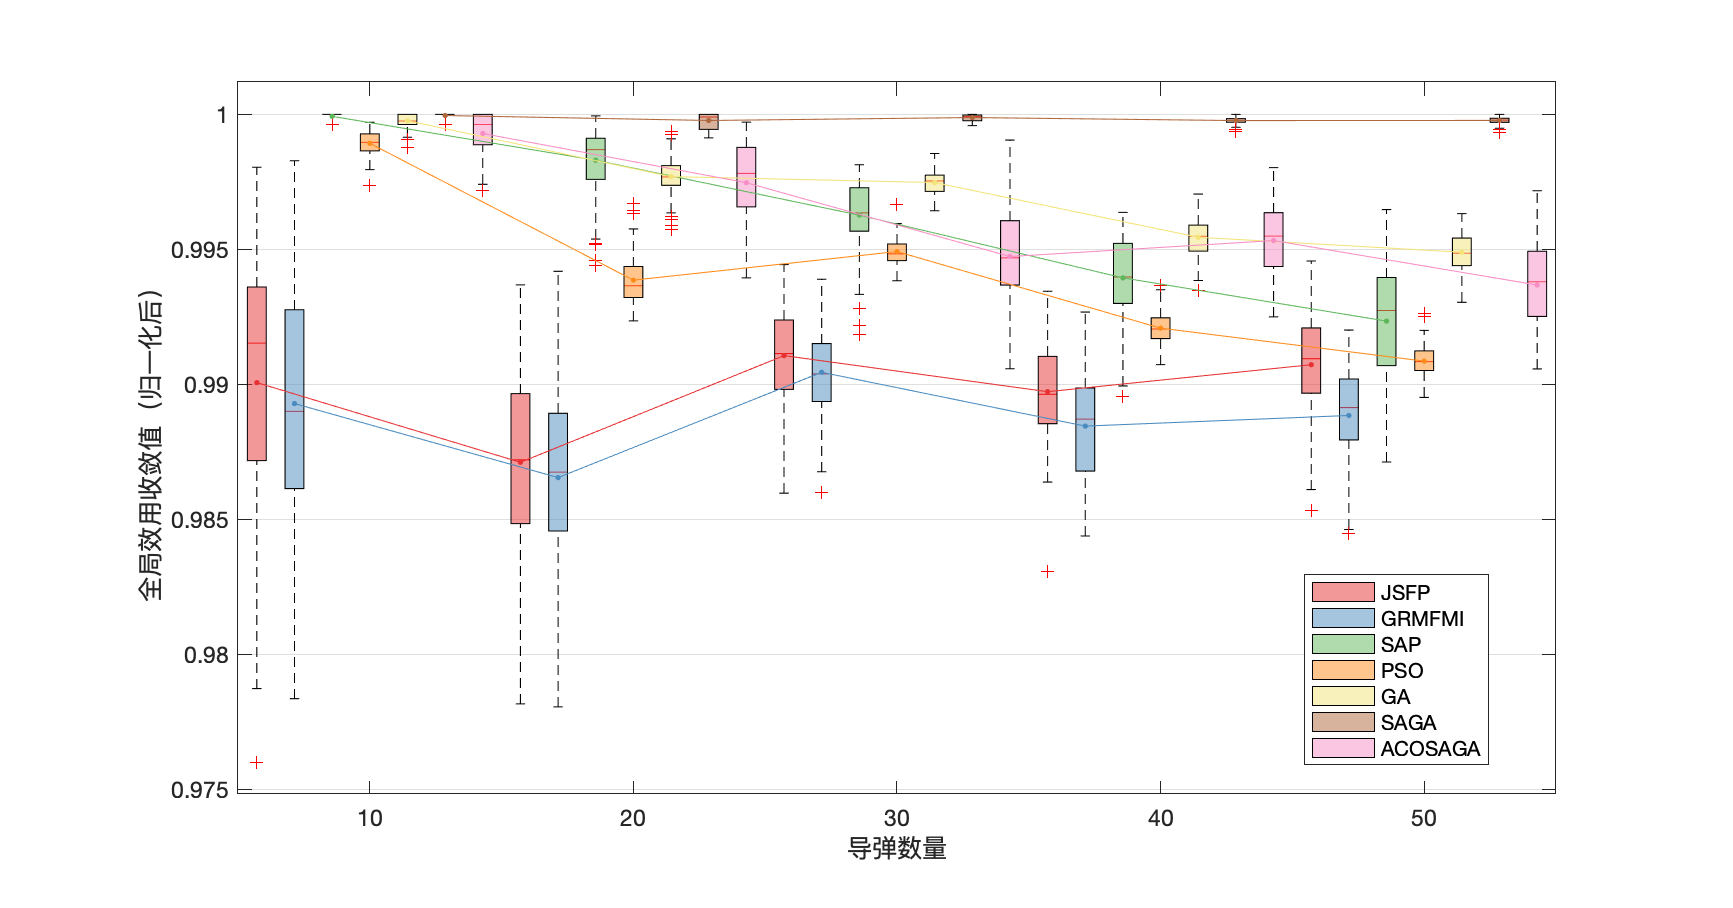
\includegraphics[height=8cm]{potential_game/BalanceBox}
  \bicaption[平衡指派场景下算法优化效果对比]
    {平衡指派场景下算法优化效果对比}
    {Comparison of performance in balance scenarios}
  \label{fig:balance}
\end{figure}

\begin{table}[!hpt]
  \bicaption[平衡指派场景下算法性能对比表]
  {平衡指派场景下算法性能对比表}
  {Comparison of algorithms' performance in balance scenarios}
  \label{tab:balance_convergence}
  \centering
  	\begin{tabular}{ccccccccc} 
  		\toprule
    \multicolumn{2}{c}{场景} & JSFP & GRMFMI & SAP & PSO & GA & SAGA & ACOSAGA\\
	\midrule
    \multirow{3}*{10vs10}  & 平均值 & 0.9901 & 0.9893 & \textbf{0.9999} & 0.9989 & 0.9998 & 1      & 0.9993\\
                           & 最大值 & 0.9980 & 0.9983 & \textbf{1}      & 0.9997 & 1      & 1      & 1     \\
                           & 最小值 & 0.9760 & 0.9783 & \textbf{0.9996} & 0.9974 & 0.9988 & 0.9996 & 0.9972\\
    \midrule
    \multirow{3}*{20vs20}  & 平均值 & 0.9871 & 0.9856 & \textbf{0.9983} & 0.9939 & 0.9977 & 0.9998 & 0.9975\\
    					   & 最大值 & 0.9937 & 0.9942 & \textbf{0.9999} & 0.9967 & 0.9994 & 1      & 0.9997\\
    					   & 最小值 & 0.9782 & 0.9780 & \textbf{0.9944} & 0.9923 & 0.9957 & 0.9991 & 0.9939\\
    \midrule
    \multirow{3}*{30vs30}  & 平均值 & 0.9911 & 0.9904 & \textbf{0.9963} & 0.9949 & 0.9975 & 0.9999 & 0.9947\\
                           & 最大值 & 0.9944 & 0.9939 & \textbf{0.9981} & 0.9966 & 0.9986 & 1      & 0.9990\\
                           & 最小值 & 0.9860 & 0.9860 & \textbf{0.9919} & 0.9938 & 0.9964 & 0.9996 & 0.9906\\
    \midrule
    \multirow{3}*{40vs40}  & 平均值 & 0.9897 & 0.9884 & \textbf{0.9939} & 0.9921 & 0.9954 & 0.9998 & 0.9953\\
                           & 最大值 & 0.9934 & 0.9927 & \textbf{0.9964} & 0.9936 & 0.9970 & 1      & 0.9980\\
                           & 最小值 & 0.9831 & 0.9844 & \textbf{0.9896} & 0.9907 & 0.9935 & 0.9994 & 0.9925\\
    \midrule
    \multirow{3}*{50vs50}  & 平均值 & 0.9907 & 0.9888 & \textbf{0.9923} & 0.9909 & 0.9949 & 0.9998 & 0.9937\\
                           & 最大值 & 0.9946 & 0.9920 & \textbf{0.9965} & 0.9926 & 0.9963 & 1      & 0.9972\\
                           & 最小值 & 0.9853 & 0.9845 & \textbf{0.9871} & 0.9895 & 0.9930 & 0.9993 & 0.9906\\
    \bottomrule
  \end{tabular}
\end{table}



\begin{figure}[!htp]
  \centering
  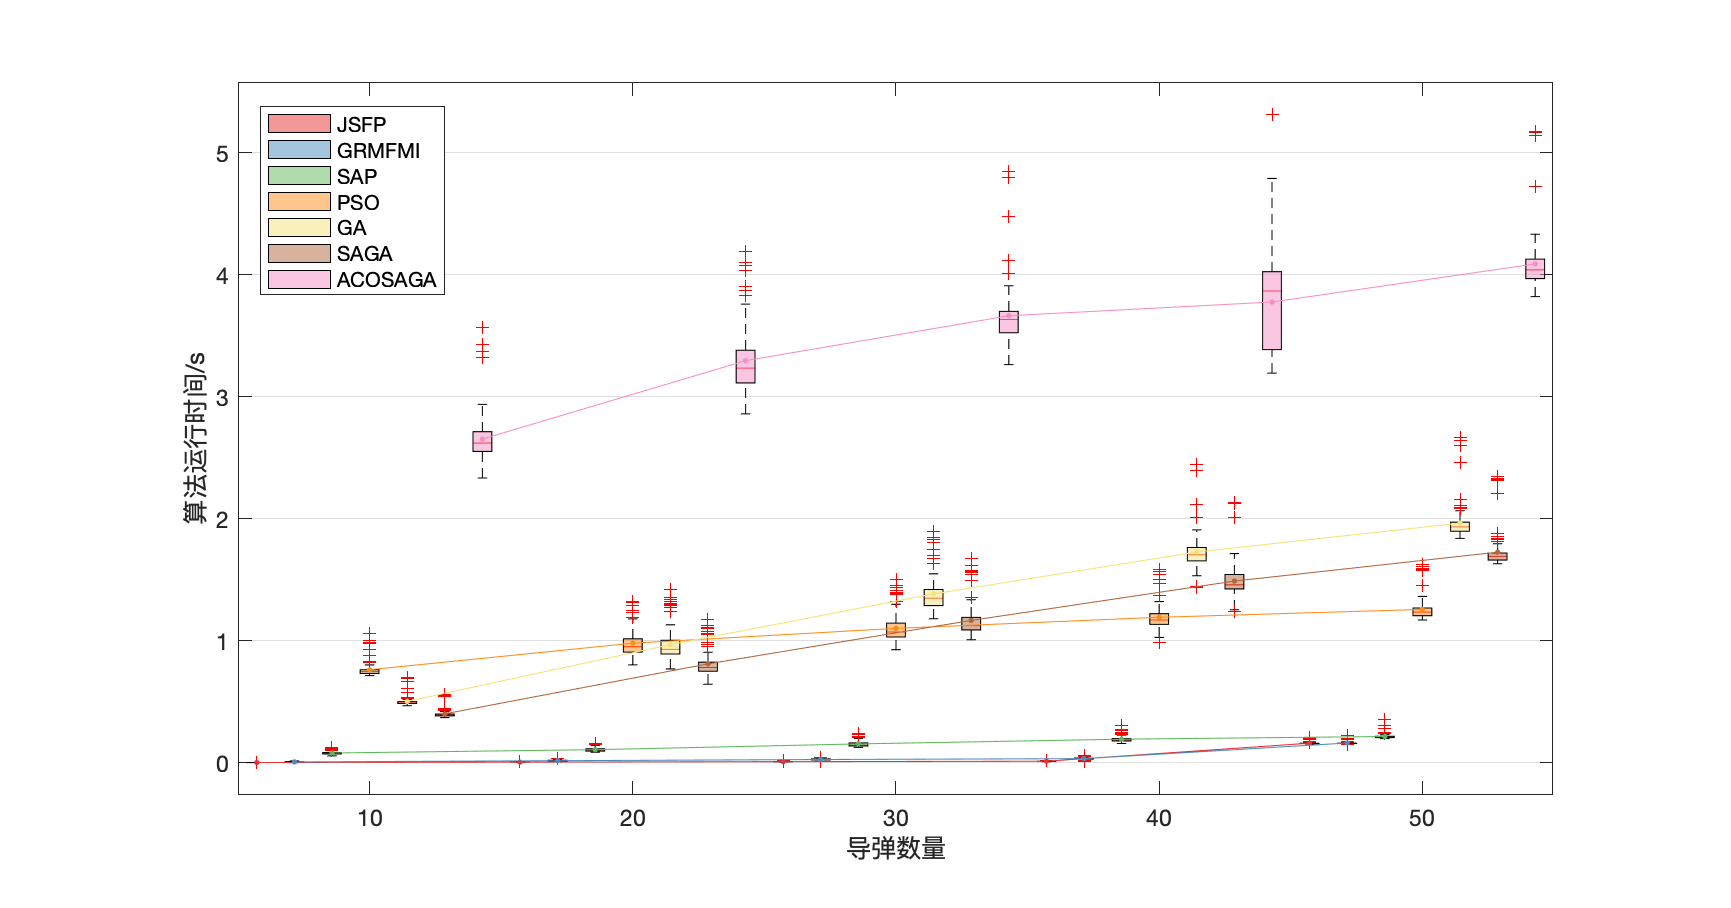
\includegraphics[height=8cm]{potential_game/BalanceBoxTime}
  \bicaption[平衡指派场景下算法运行时间对比]
    {平衡指派场景下算法运行时间对比}
    {Comparison of running time in balance scenarios}
  \label{fig:balance_time}
\end{figure}



  
  \begin{table}[!hpt]
  \bicaption[平衡指派场景下算法运行时间对比表]
  {平衡指派场景下算法运行时间对比表(单位:s)}
  {Table of comparison of algorithms' running time in balance scenarios (unit: s)}
  \label{tab:balance_time}
  \centering
	\begin{tabular}{ccccccccc} 
  		\toprule
    \multicolumn{2}{c}{场景} & JSFP & GRMFMI & SAP & PSO & GA & SAGA & ACOSAGA\\
	\midrule
    \multirow{3}*{10vs10}  & 平均值 & 0.0020 & 0.0070 & 0.0801 & 0.7627 & 0.5033 & 0.4010 & 2.6535\\
                           & 最大值 & 0.0031 & 0.0153 & 0.1241 & 1.0614 & 0.7026 & 0.5615 & 3.5692\\
                           & 最小值 & 0.0015 & 0.0019 & 0.0565 & 0.7140 & 0.4676 & 0.3706 & 2.3345\\
    \midrule
    \multirow{3}*{20vs20}  & 平均值 & 0.0055 & 0.0170 & 0.1073 & 0.9803 & 0.9686 & 0.8107 & 3.2959\\
    					   & 最大值 & 0.0108 & 0.0343 & 0.1618 & 1.3223 & 1.4168 & 1.1736 & 4.1926\\
    					   & 最小值 & 0.0036 & 0.0056 & 0.0861 & 0.8024 & 0.7690 & 0.6435 & 2.8598\\
    \midrule
    \multirow{3}*{30vs30}  & 平均值 & 0.0092 & 0.0268 & 0.1547 & 1.1018 & 1.3845 & 1.1669 & 3.6641\\
                           & 最大值 & 0.0160 & 0.0462 & 0.2434 & 1.5053 & 1.8977 & 1.6706 & 4.8505\\
                           & 最小值 & 0.0067 & 0.0087 & 0.1263 & 0.9268 & 1.1805 & 1.0086 & 3.2637\\
    \midrule
    \multirow{3}*{40vs40}  & 平均值 & 0.0127 & 0.0339 & 0.1933 & 1.1925 & 1.7278 & 1.4894 & 3.7765\\
                           & 最大值 & 0.0194 & 0.0557 & 0.3036 & 1.5871 & 2.4452 & 2.1338 & 5.3144\\
                           & 最小值 & 0.0085 & 0.0136 & 0.1580 & 0.9871 & 1.4368 & 1.2369 & 3.1942\\
    \midrule
    \multirow{3}*{50vs50}  & 平均值 & 0.1604 & 0.1620 & 0.2154 & 1.2572 & 1.9641 & 1.7263 & 4.0889\\
                           & 最大值 & 0.2101 & 0.2267 & 0.3529 & 1.6237 & 2.6694 & 2.3463 & 5.1781\\
                           & 最小值 & 0.1540 & 0.1493 & 0.1977 & 1.1702 & 1.8390 & 1.6316 & 3.8209\\
    \bottomrule
  \end{tabular}
\end{table}

首先针对平衡指派场景进行分析,设置导弹或目标数量从10增加到50,在这五种场景下使用本章介绍的三种算法在内的七种算法,独立重复进行100次优化。

本文使用的仿真平台是Ubuntu16.04系统下的Matlab R2018a。图\ref{fig:balance}展示的是得到的收敛值分布箱型图及其平均值曲线,具体平均值、最大值和最小值数据见表\ref{tab:balance_convergence},表中加粗数据为本章使用的三种算法中的最大值。图\ref{fig:balance_time}展示的是七种算法完成一次优化求解的运行时间的分布箱型图及其平均值曲线,具体平均值、最大值和最小值数据见表\ref{tab:balance_time}。其中由于分布式架构,JSFP和GRMFMI算法的运行时间是按照所有导弹完成一次迭代后的总时间除以导弹数量作为算法一次迭代的运行时间,而SAP算法由于在一次迭代中只有一枚导弹参与迭代,因此不需要进行此操作。


从同个场景下的算法之间的对比角度分析,由图\ref{fig:balance}和表\ref{tab:balance_convergence}中可看出,在优化效果方面,在五种场景下,所有算法基本可以找到较优解,最差优化结果也达到了最好结果的97.5\%以上。具体而言,SAGA算法效果最好,基本在所有场景下都得到了七种算法的最大值,其次为GA算法,SAP和ACOSAGA算法效果相当,接着为PSO算法,最后为JSFP和GRMFMI,两者效果相近,即在优化结果方面顺序为:SAGA>GA>ACOSAGA$\approx$SAP>PSO>JSFP$\geq$GRMFMI。在收敛结果分散程度方面,SAGA算法仍然是表现最优的算法,其重复实验的结果十分集中,GA和PSO算法其次,SAP和ACOSAGA算法分散程度相当,甚至在导弹数量为10和20时比ACOSAGA更集中,JSFP和GRMFMI仍然是排在最后的算法。因此在收敛结果分散程度方面的排序为:SAGA>GA$\approx$PSO>SAP$\approx$ACOSAGA>GRMFMI$\approx$JSFP,但需要指出的是,考虑到此处结果的幅值范围很小,实际上即使是最分散的情况下,比如JSFP算法在10个目标的场景下,优化最大值与最小值相差只有0.022。

从不同场景角度分析,随着任务分配规模的扩大,集中式算法除了SAGA外,优化效果都有略微下降。分析本章使用的三种博弈学习算法,可以看出当问题规模较小时,SAP算法可以达到与集中式算法相当的优化效果,但随着导弹数量的增加,此时由于SAP算法机制中每次只有一个智能体进行决策,使得不能完全探索策略空间,因此相对来说性能有所下降;相反地,JSFP算法和GRMFMI算法在导弹数量增加后反而表现有所提高,甚至接近了SAP算法,但距离集中式算法的效果还有一定距离。分析认为这是由于JSFP算法和GRMFMI算法在每次迭代都会让所有智能体选出最优决策,虽然是以一定概率采纳,但在面对较大的策略空间时,相比SAP更能搜索到更优解。

由图\ref{fig:balance_time}和表\ref{tab:balance_time}中的时间数据可看出,由于分布式架构的作用,JSFP、GRMFMI和SAP算法的运行时间几乎不受导弹数量的影响,其他六种算法的运行时间随着导弹数量的增加都有所增加,其中ACOSAGA算法运行时间最长。由于分布式架构的优势,JSFP、GRMFMI和SAP算法在五种场景下耗时几乎不变,且均为运行最快的算法。此外,这三种算法运行时间较为集中,而其他算法均或多或少存在耗时较长的的特殊运行场景。特别需要指出的是,虽然这里没有将导弹之间的通信一致性过程耗费时间考虑在内。但由于SAP算法在每次迭代中只有一个导弹进行决策,因此在通信方面与集中式算法消耗的资源与时间是相当的,在此前提下SAP算法仍具有更好的实时性。

综上所述,本章使用的三种博弈论学习算法均兼具了良好的优化效果,但在优化结果的集中程度方面略差于集中式算法。若将运行时间纳入综合考虑,则本章介绍的基于势博弈模型及其学习算法的任务分配方法在求解规模较大的任务分配问题时具有突出的时间优势,且相比于集中式算法的优化效果减弱程度处于可以接受的范围内。


\subsection{非平衡指派场景仿真分析}
\label{pg:sim:unbalance}
接着,固定导弹数量为55,目标数量从10增加到50,在不能平分导弹的场景下,会有部分目标所需的导弹数量较大,本节设置的场景是使得目标所需的导弹数量尽量接近\footnote{第\ref{chap:hedonic}章的\ref{hg:sec:simulation}小节中将对非平衡指派场景做进一步深入说明和研究。} 。仍然使用上述七种算法对这五种场景进行独立重复100次优化。正如前文所说,集中式启发算法会事先通过增设虚拟目标的方法,将不平衡指派问题转化为平衡指派问题,而本章使用的基于势博弈模型的分布式算法则不需要进行此操作。下面将分析在不平衡分配问题下本章使用的博弈学习算法的有效性。

图\ref{fig:unbalance}展示的是100次优化结果下收敛值的分布箱型图及其平均值曲线,具体平均值、最大值和最小值数据见表\ref{tab:unbalance_convergence}。图\ref{fig:unbalance_time}展示的是七种算法得到最终收敛解的运行时间分布式箱型图及其平均值曲线,与\ref{pg:sim:balance}小节一样,JSFP和GRMFMI的运行时间是由一次求解的总运行时间除以导弹数量得到的平均时间。具体运行时间的平均值、最大值和最小值数据见表\ref{tab:unbalance_time}。

由图\ref{fig:unbalance}和表\ref{tab:unbalance_convergence}数据可看出,在不平衡指派问题中,本章使用的势博弈模型下的三种算法在大多数优化中均能够达到集中式算法最好效果的98\%以上,其中JSFP和SAP算法在一些场景下优化效果比PSO算法更好,但GRMFMI算法相对来说是三种算法中表现较差的。因此七种算法的优化排序为SAGA>GA>ACOSAGA>PSO$\approx$SAP$\approx$JSFP>GRMFMI。在优化的分散程度方面,势博弈模型下的三种算法相比较集中式算法而言,多次优化的收敛结果较为分散,但从分散的绝对程度来看这样的分散程度是很小的,比如GRMFMI算法在五种场景下优化的最大值和最小值相差最大幅度为0.013。

此外,从不同场景来看,在不同的非平衡场景中,三种势博弈学习算法的性能随着目标数增加略有下降但下降幅度只在0.01范围内,几乎可以认为不变。可见三种学习算法对于非平衡分配问题的求解依然保持着较好的性能。

\begin{figure}[!htp]
  \centering
  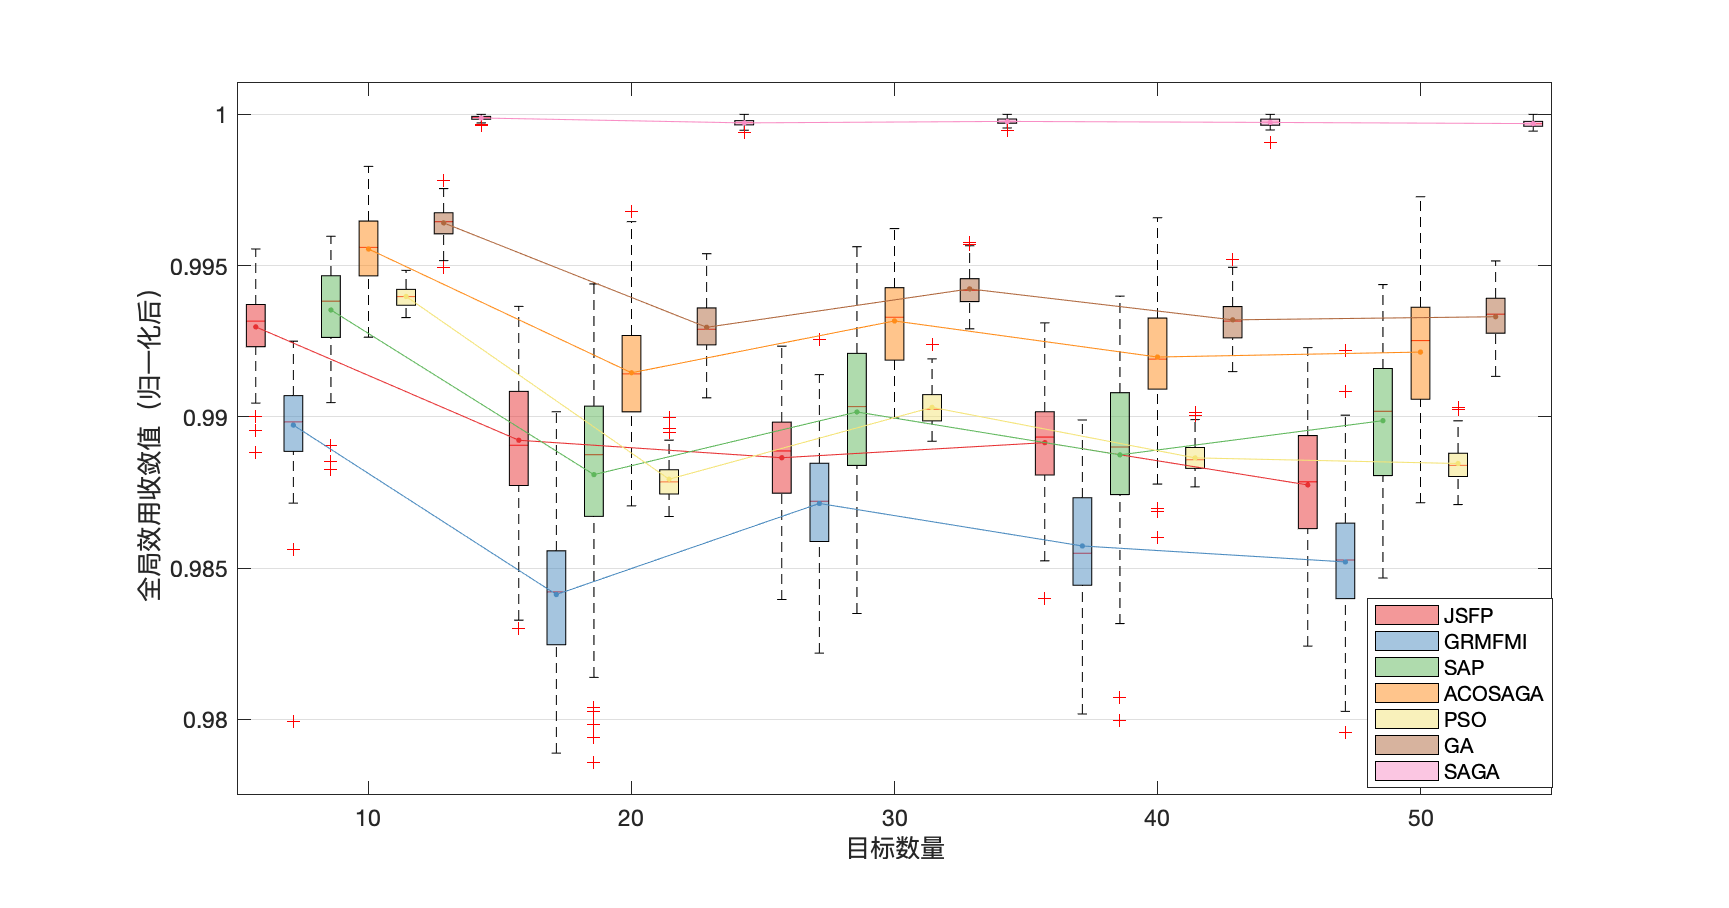
\includegraphics[height=8cm]{potential_game/BoxM55T10-50}
  \bicaption[固定导弹数量为55非平衡指派场景下算法优化效果对比]
    {固定导弹数量为55非平衡指派场景下算法优化效果对比}
    {Comparison of performance in unbalance scenarios with 55 missiles}
  \label{fig:unbalance}
\end{figure}




\begin{table}[!hpt]
  \bicaption[固定导弹数量为55非平衡指派场景下算法性能对比表]
  {固定导弹数量为55非平衡指派场景下算法性能对比表}
  {Comparison of algorithms' performance in unbalance scenarios with 55 missiles}
  \label{tab:unbalance_convergence}
  \centering
  	\begin{tabular}{ccccccccc} 
  		\toprule
    \multicolumn{2}{c}{场景} & JSFP & GRMFMI & SAP & PSO & GA & SAGA & ACOSAGA\\
	\midrule
    \multirow{3}*{55vs10}  & 平均值 & 0.9930 & 0.9897 & \textbf{0.9935} & 0.9940 & 0.9964 & 0.9999 & 0.9956\\
                           & 最大值 & 0.9956 & 0.9925 & \textbf{0.9960} & 0.9948 & 0.9978 & 1      & \underline{0.9983}\\
                           & 最小值 & \textbf{0.9888} & 0.9799 & 0.9883 & 0.9933 & 0.9949 & 0.9996 & 0.9926\\
    \midrule
    \multirow{3}*{55vs20}  & 平均值 & \textbf{0.9892} & 0.9841 & 0.9881 & 0.9879 & 0.9930 & 0.9997 & 0.9915\\
    					   & 最大值 & 0.9937 & 0.9902 & \textbf{0.9944} & 0.9900 & 0.9954 & 1      & \underline{0.9968}\\
    					   & 最小值 & \textbf{0.9830} & 0.9789 & 0.9786 & 0.9867 & 0.9906 & 0.9994 & 0.9871\\
    \midrule
    \multirow{3}*{55vs30}  & 平均值 & 0.9887 & 0.9871 & \textbf{0.9902} & 0.9903 & 0.9942 & 0.9998 & 0.9932\\
                           & 最大值 & 0.9923 & 0.9926 & \textbf{0.9956} & 0.9924 & 0.9958 & 1      & 0.9962\\
                           & 最小值 & \textbf{0.9840} & 0.9822 & 0.9835 & 0.9892 & 0.9929 & 0.9995 & 0.9900\\
    \midrule
    \multirow{3}*{55vs40}  & 平均值 & \textbf{0.9892} & 0.9857 & 0.9887 & 0.9886 & 0.9932 & 0.9997 & 0.9920\\
                           & 最大值 & 0.9931 & 0.9899 & \textbf{0.9940} & 0.9901 & 0.9952 & 1      & 0.9966\\
                           & 最小值 & \textbf{0.9840} & 0.9802 & 0.9800 & 0.9877 & 0.9915 & 0.9991 & 0.9860\\
    \midrule
    \multirow{3}*{55vs50}  & 平均值 & 0.9878 & 0.9852 & \textbf{0.9899} & 0.9885 & 0.9933 & 0.9997 & 0.9921\\
                           & 最大值 & 0.9923 & 0.9922 & \textbf{0.9944} & 0.9903 & 0.9952 & 1      & 0.9973\\
                           & 最小值 & 0.9824 & 0.9796 & \textbf{0.9847} & 0.9871 & 0.9913 & 0.9994 & 0.9872\\
    \bottomrule
  \end{tabular}
\end{table}


\begin{figure}[!htp]
  \centering
  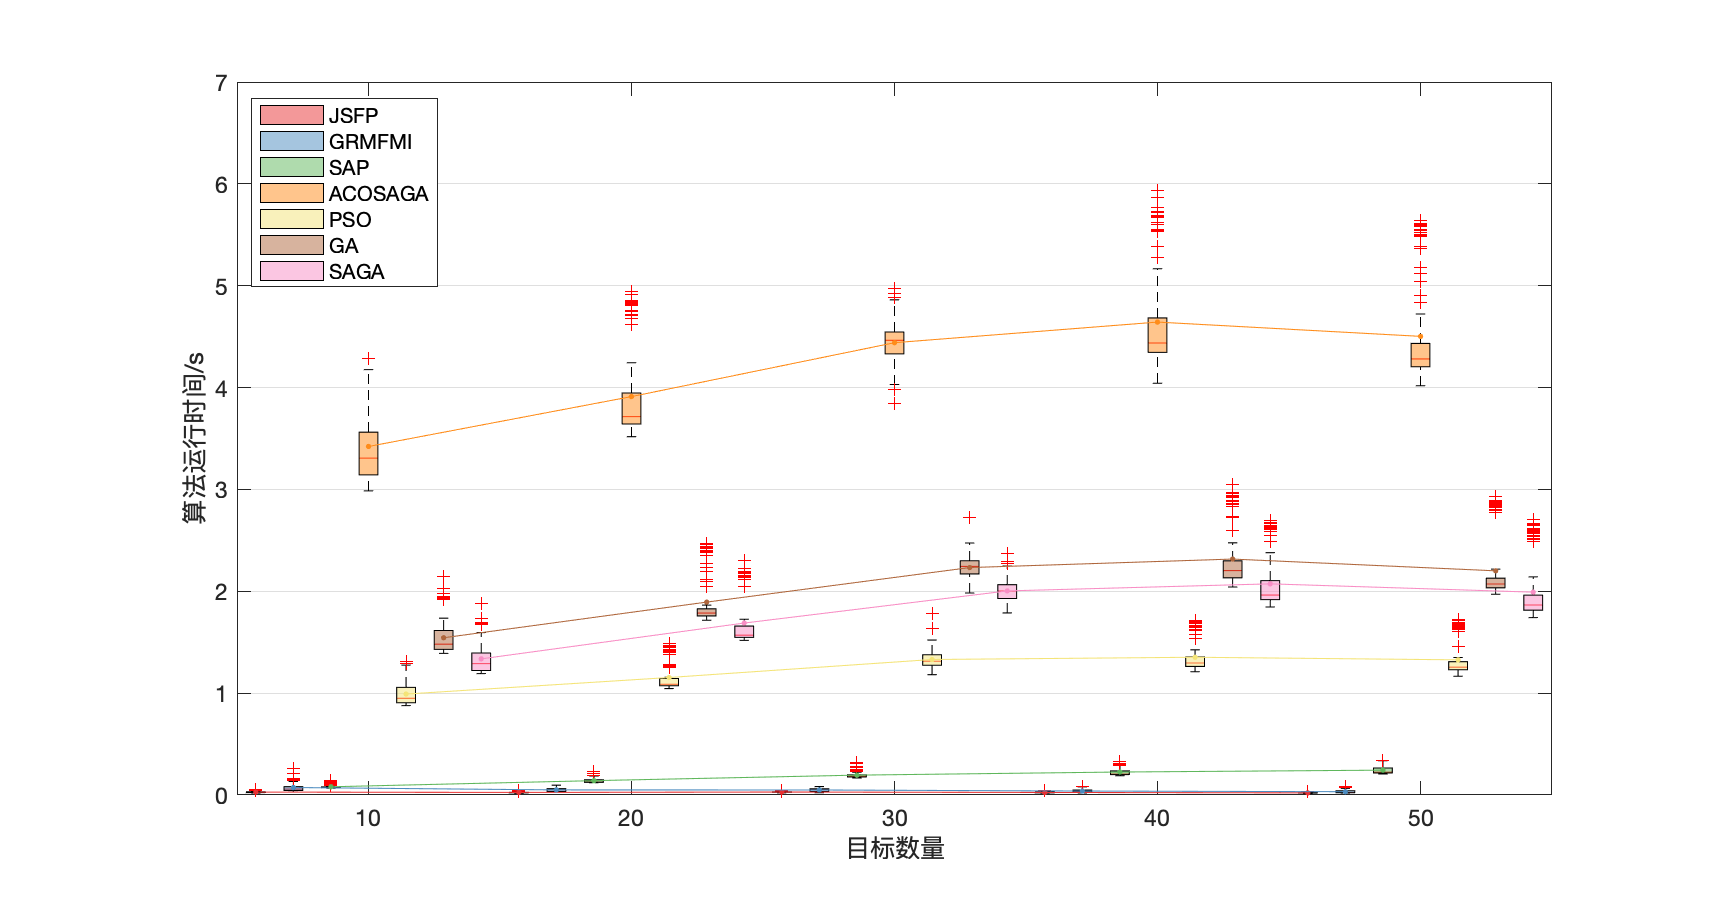
\includegraphics[height=8cm]{potential_game/BoxM55T10-50Time}
  \bicaption[固定导弹数量为55的非平衡指派场景下算法运行时间对比]
    {固定导弹数量为55的非平衡指派场景下算法运行时间对比}
    {Comparison of running time in unbalance scenarios with 55 missiles}
  \label{fig:unbalance_time}
\end{figure}



\begin{table}[!hpt]
  \bicaption[固定导弹数量为55的非平衡指派场景下算法运行时间对比表]
  {固定导弹数量为55的非平衡指派场景下算法运行时间对比表(单位:s)}
  {Comparison of running time in unbalance scenarios with 55 missiles (unit: s)}
  \label{tab:unbalance_time}
  \centering
  	\begin{tabular}{ccccccccc} 
  		\toprule
    \multicolumn{2}{c}{场景} & JSFP & GRMFMI & SAP & PSO & GA & SAGA & ACOSAGA\\
	\midrule
    \multirow{3}*{55vs10}  & 平均值 & 0.0286 & 0.0733 & 0.0807 & 0.9909 & 1.5437 & 1.3366 & 3.4217\\
                           & 最大值 & 0.0564 & 0.2566 & 0.1422 & 1.3096 & 2.1459 & 1.8846 & 7.4429\\
                           & 最小值 & 0.0180 & 0.0289 & 0.0664 & 0.8778 & 1.3902 & 1.1920 & 2.9859\\
    \midrule
    \multirow{3}*{55vs20}  & 平均值 & 0.0253 & 0.0499 & 0.1409 & 1.1535 & 1.8938 & 1.6882 & 3.9115\\
    					   & 最大值 & 0.0439 & 0.0964 & 0.2298 & 1.4860 & 2.4671 & 2.3054 & 4.9388\\
    					   & 最小值 & 0.0166 & 0.0276 & 0.1200 & 1.0448 & 1.7158 & 1.5182 & 3.5176\\
    \midrule
    \multirow{3}*{55vs30}  & 平均值 & 0.0291 & 0.0492 & 0.1950 & 1.3303 & 2.2328 & 2.0036 & 4.4405\\
                           & 最大值 & 0.0396 & 0.0829 & 0.3142 & 1.7790 & 2.7263 & 2.3679 & 4.9753\\
                           & 最小值 & 0.0212 & 0.0223 & 0.1674 & 1.1810 & 1.9835 & 1.7875 & 3.8433\\
    \midrule
    \multirow{3}*{55vs40}  & 平均值 & 0.0250 & 0.0389 & 0.2256 & 1.3524 & 2.3164 & 2.0730 & 4.6430\\
                           & 最大值 & 0.0421 & 0.0838 & 0.3337 & 1.7167 & 3.0509 & 2.6925 & 5.9372\\
                           & 最小值 & 0.0175 & 0.0195 & 0.1890 & 1.2101 & 2.0421 & 1.8454 & 4.0420\\
    \midrule
    \multirow{3}*{55vs50}  & 平均值 & 0.0208 & 0.0323 & 0.2439 & 1.3269 & 2.2009 & 1.9915 & 4.5028\\
                           & 最大值 & 0.0334 & 0.0838 & 0.3408 & 1.7194 & 2.9258 & 2.7018 & 5.6404\\
                           & 最小值 & 0.0152 & 0.0187 & 0.2062 & 1.1657 & 1.9712 & 1.7415 & 4.0176\\
    \bottomrule
  \end{tabular}
\end{table}


在运行时间方面,由图\ref{fig:unbalance_time}和表\ref{tab:unbalance_time}可知,类似于\ref{pg:sim:balance}中的分析结果,本章使用的三种分布式算法在实时性方面比集中式算法更具优势,且几乎不会随着问题规模的改变而产生变化。

综上所述,针对非平衡指派问题,本章使用的势博弈模型及三种博弈学习算法可以获得良好而稳定的效果,且相较于集中式算法,不需要事先对非平衡问题进行转换。在实时性方面,三种算法仍然具有分布式架构下的突出的实时性优势。

\section{本章小结}
\label{pg:conclusion}

本章阐述了基于势博弈模型和学习算法的分布式任务分配方法。首先介绍了势博弈模型的概念,并利用WLU效用函数建立起势博弈模型。接着针对任务分配问题中的约束条件,引入了分布化的Lagrange乘子,对WLU效用函数进行修正,从理论上证明了基于修正后的WLU函数的智能体效用的可行性以及性能下界。之后本章介绍了三种势博弈模型下的学习算法,并提出了任务交易机制,对SAP算法进行了改进。最后通过仿真验证了势博弈模型在平衡和非平衡任务分配场景下的有效性,及其学习算法优良的实时性。





















